\documentclass{VUMIFInfKursinis}
\usepackage{algorithmicx}
\usepackage[linesnumbered,ruled,vlined]{algorithm2e}
\usepackage{caption}
\usepackage{amsfonts}
\usepackage{amsmath}
\usepackage{tikz}
\usepackage{pgfplots}
\usepackage{bm}
\usepackage{color}
\usepackage{graphicx}
\usepackage{float}
\usepackage{xcolor}
\usepackage{hyperref}
\usepackage{url}


% Titulinio aprašas
\university{Vilniaus universitetas}
\faculty{Matematikos ir informatikos fakultetas}
\institute{Informatikos institutas}
\department{Informatikos katedra}
\papertype{Projektinis Darbas}
\title{Visų maksimalių grafo klikų generavimas}
\titleineng{Generating all maximal cliques}
\status{3 kurso 2 grupės studentas}
\author{Ričardas Čubukinas}
\supervisor{Asist., Dr. Valdas Dičiūnas}

\makeatletter
\def\BState{\State\hskip-\ALG@thistlm}
\makeatother

\date{Vilnius \\ \the\year}

% Nustatymai
\setmainfont{Palem}[
  Extension = .ttf,
  Path = Palemonas/,
  UprightFont = *-nm,
  BoldFont  = *-bd ,
  ItalicFont  = *-it ,
  BoldItalicFont = *-bi ]
%\setmainfont{Palemonas}
\bibliography{bibliografija} 
\renewcommand{\algorithmcfname}{Algoritmas}

\begin{document}
\maketitle

\tableofcontents

\sectionnonum{Problemos formulavimas}
\begin{itemize}
  \item{\textbf{Duota:} Neorientuotas grafas $G=(V,E)$, turintis $n$ viršūnių ir $m$ briaunų.}
  \item{\textbf{Rasti:} Visas maksimalias grafo G klikas, t.y. tokius viršūnių aibės poaibius kurie grafe $G$ sudaro pilną pografį ir kurių nebegalima praplėsti taip, kad vėl gautųsi pilnas pografis.}
\end{itemize}

Realizuoti visų grafo klikų paieškos su grįžimu atgal („backtracking“) algoritmą ir ištirti jo
sudėtingumą:
\begin{enumerate}
  \item{Teoriškai.}
  \item{Praktiškai kaip priklauso nuo grafo viršūnių skaičiaus $n$ ir briaunų skaičiaus $m$.}
\end{enumerate}

\section{Algoritmas}
Bron-Kerbosch algoritmo forma yra rekursinis grįžtamasis(„backtracking“) algoritmas, kuriuo ieškoma visų maksimalių klikų duotame grafe $G$. Esant trims nesujungtoms viršūnių aibėms $R$, $P$ ir $X$, randamos maksimalios klikos, į kurias įeina visos $R$ viršūnės, kai kurios $P$ viršūnės ir nė viena $X$ viršūnė. Kiekvieno algoritmo iškvietimo metu $P$ ir $X$ yra nesujungtos aibės, kurių sąjungą sudaro tos viršūnės, kurios, pridėjus jas prie R, sudaro kliką. Kitaip tariant, $P \cup X$ yra aibė viršūnių, kurios yra sujungtos su kiekvienu $R$ elementu.

Rekursija pradedama nustatant, kad $R$ ir $X$ yra tuščia aibė, o $P$ - grafo viršūnių aibė. Per kiekvieną rekursinį iškvietimą algoritmas paeiliui nagrinėja $P$ viršūnes; jei tokių viršūnių nėra, jis arba praneša, kad $R$ yra maksimali klika (jei $X$ tuščia), arba grįžta atgal. Kiekvienai viršūnei $v$, pasirinktai iš $P$, algoritmas atlieka pasikartojantį iškvietimą, per kurį $v$ pridedama prie $R$ ir per kurį $P$ ir $X$ apsiriboja $v$ kaimynų aibe $N(v)$, kurioje surandami ir pranešami visi $R$ klikos plėtiniai, kuriuose yra $v$. Tada $v$ perkeliama iš $P$ į $X$, kad į ją nebūtų atsižvelgta būsimuose klikose, ir tęsiamas darbas su kita $P$ viršūne. 

Tačiau aprašyta pagrindinė algoritmo forma yra neefektyvi, kai grafai turi daug nemaksimalių klikų: kiekvienai klikai, nesvarbu, ar ji maksimali, ar ne, atliekamas rekursinis iškvietimas. Siekdami sutaupyti laiko ir leisti algoritmui greičiau grįžti į paieškos šakas, kuriose nėra maksimalių klikų, Bron ir Kerbosch įvedė algoritmo variantą, apimantį "atsparos tašką" $u$, parinktą iš iš $P \cup X$. Bet kurioje maksimalioje klikoje turi būti arba $u$, arba vienas iš jos neesančių kaimynų, nes priešingu atveju klika galėtų būti padidinta į ją įtraukus $u$. Todėl kiekviename algoritmo rekursyviame iškvietime į $R$ pridedamos viršūnės $v$ pasirinkimo variantai turi būti tikrinami tik $u$ ir jos ne kaimynės.

\begin{algorithm}[H]
  \DontPrintSemicolon
  \caption{Bron Kerbosch su atsparos tašku}
  \textbf{Duomenys:} Neorientuotas grafas $G=(V,E)$ \;
  \textbf{Rezultatas:} Visos maksimalios grafo $G$ klikos \;
  $P \gets V$ \;
  $N \gets \emptyset$ \;
  \ForEach{briauna $e_i, e_j$ $\in$ E}{
    $N[e_i] \gets N[e_i] + e_j$ \;
    $N[e_j] \gets N[e_j] + e_i$ \;
  }
  \SetKwFunction{FMain}{generuoti\_maksimalias\_klikas}
  \SetKwProg{Fn}{Function}{:}{}
  \Fn{\FMain{$P$, $R$, $X$}}{
    \If{$P$ and $X$ \textbf{not} $\emptyset$}{
      paskelbti R kaip maksimalią kliką  \;
    }
      parenkame atsparos tašką - briauną $u$ iš $P \cap X$ \;
      \ForEach{briauna $v$ $\in$ $P \setminus N(u)$}{
       \FMain{$P$ $\cap$ $N(v)$, $R$ $\cup$ $\{v\}$, $X$ $\cap$ $N(v)$} \;
       $P \gets P \setminus \{v\}$ \;
       $X \gets X \setminus \{v\}$ \;
      }
    
  }
\end{algorithm}

% Eksperimentavimas su skirtingais duomenimis vykdymo laikas ats ir t.t
\section{Eksperimentai}
\subsection{Grafas 1}
\begin{figure}[H]
  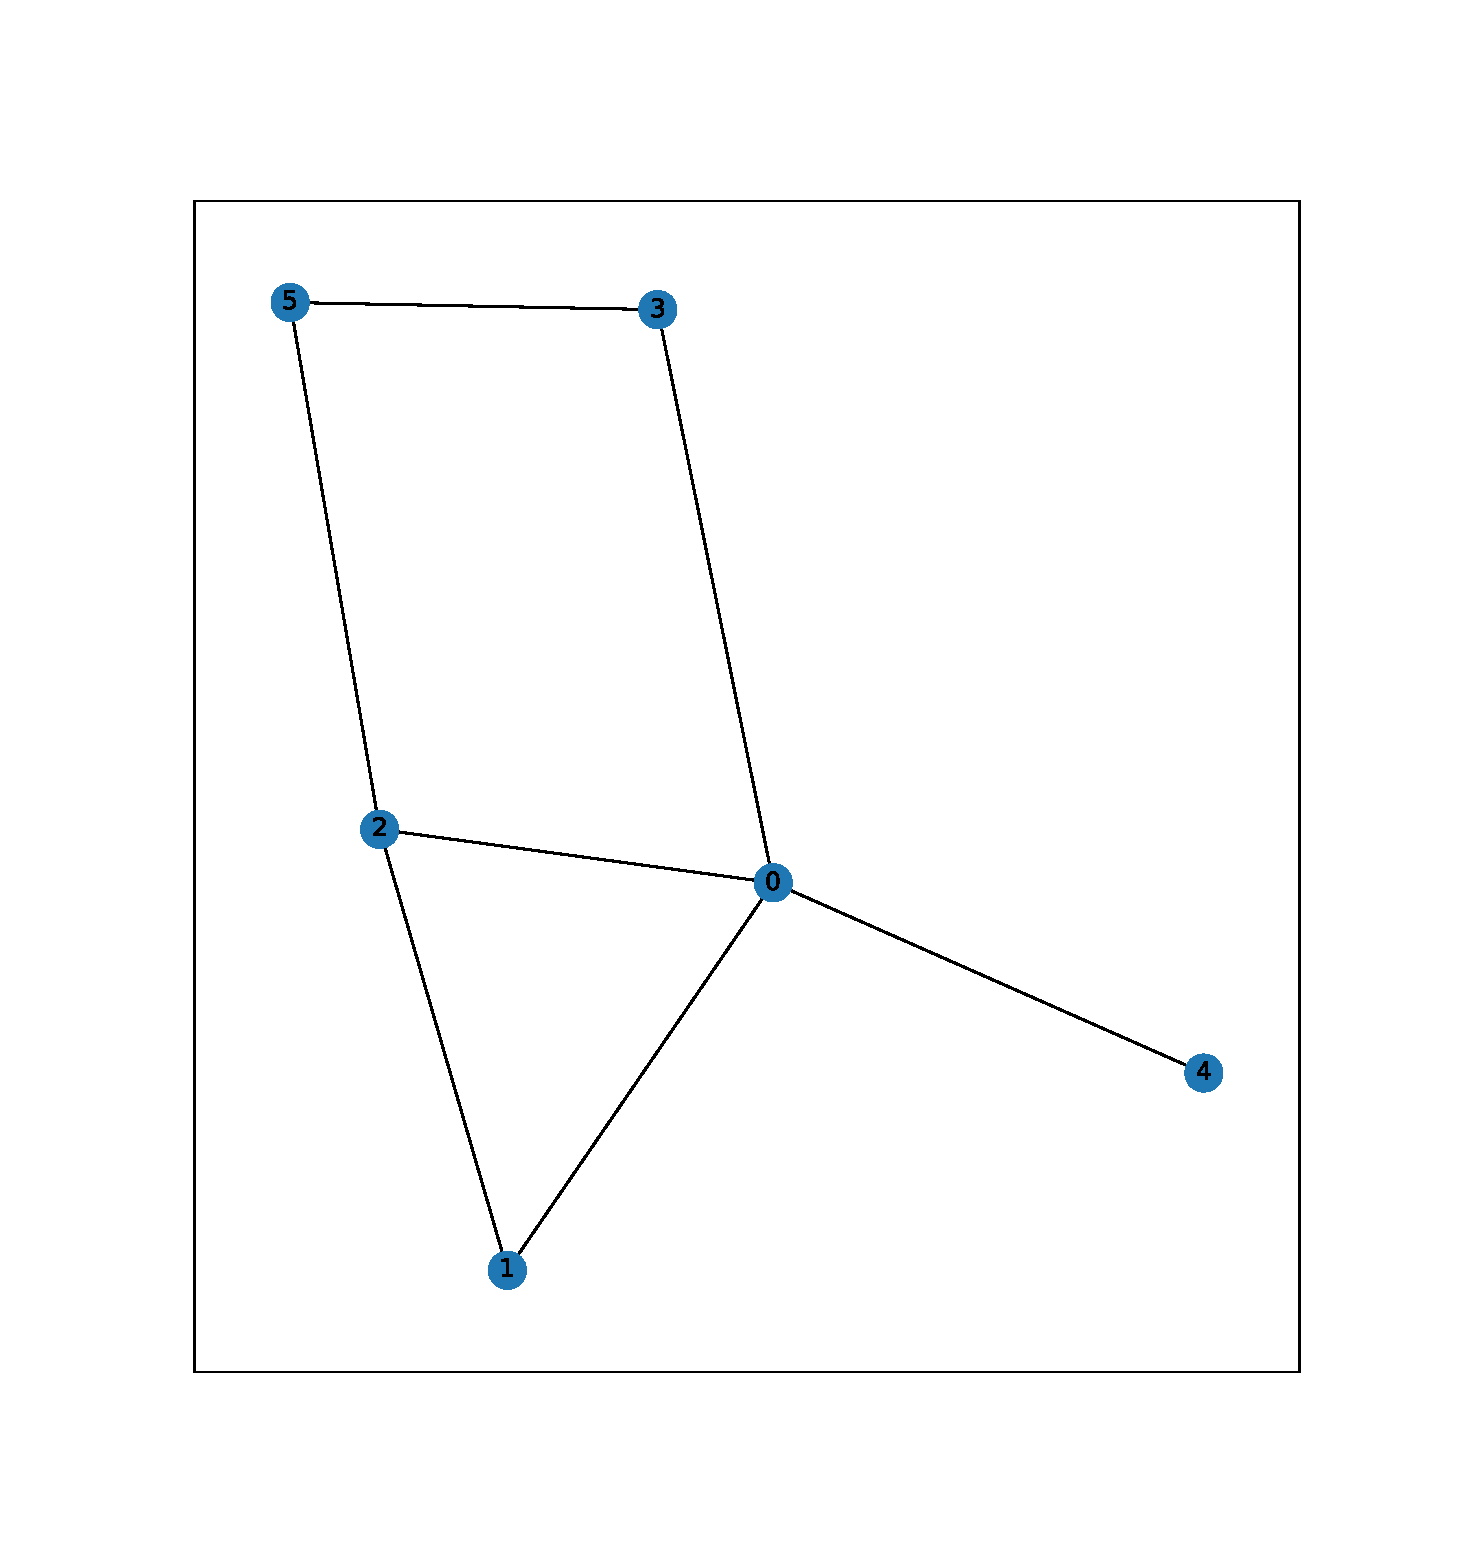
\includegraphics[height=0.7\textwidth,width=0.7\textwidth]{img/graph_1.eps}
\end{figure}

\begin{verbatim}
Duomenys:
n = 6 viršūnės, m = 7 briaunos.
V = [0, 1, 2, 3, 4, 5]
E = [(0, 1), (0, 2), (0, 3), (0, 4), (1, 2), (2, 5), (3, 5)]
Sugeneruotos maksimalios klikos:
[{0, 1, 2}, {0, 3}, {0, 4}, {2, 5}, {3, 5}]
\end{verbatim}


\subsection{Grafas 2}
\begin{figure}[H]
  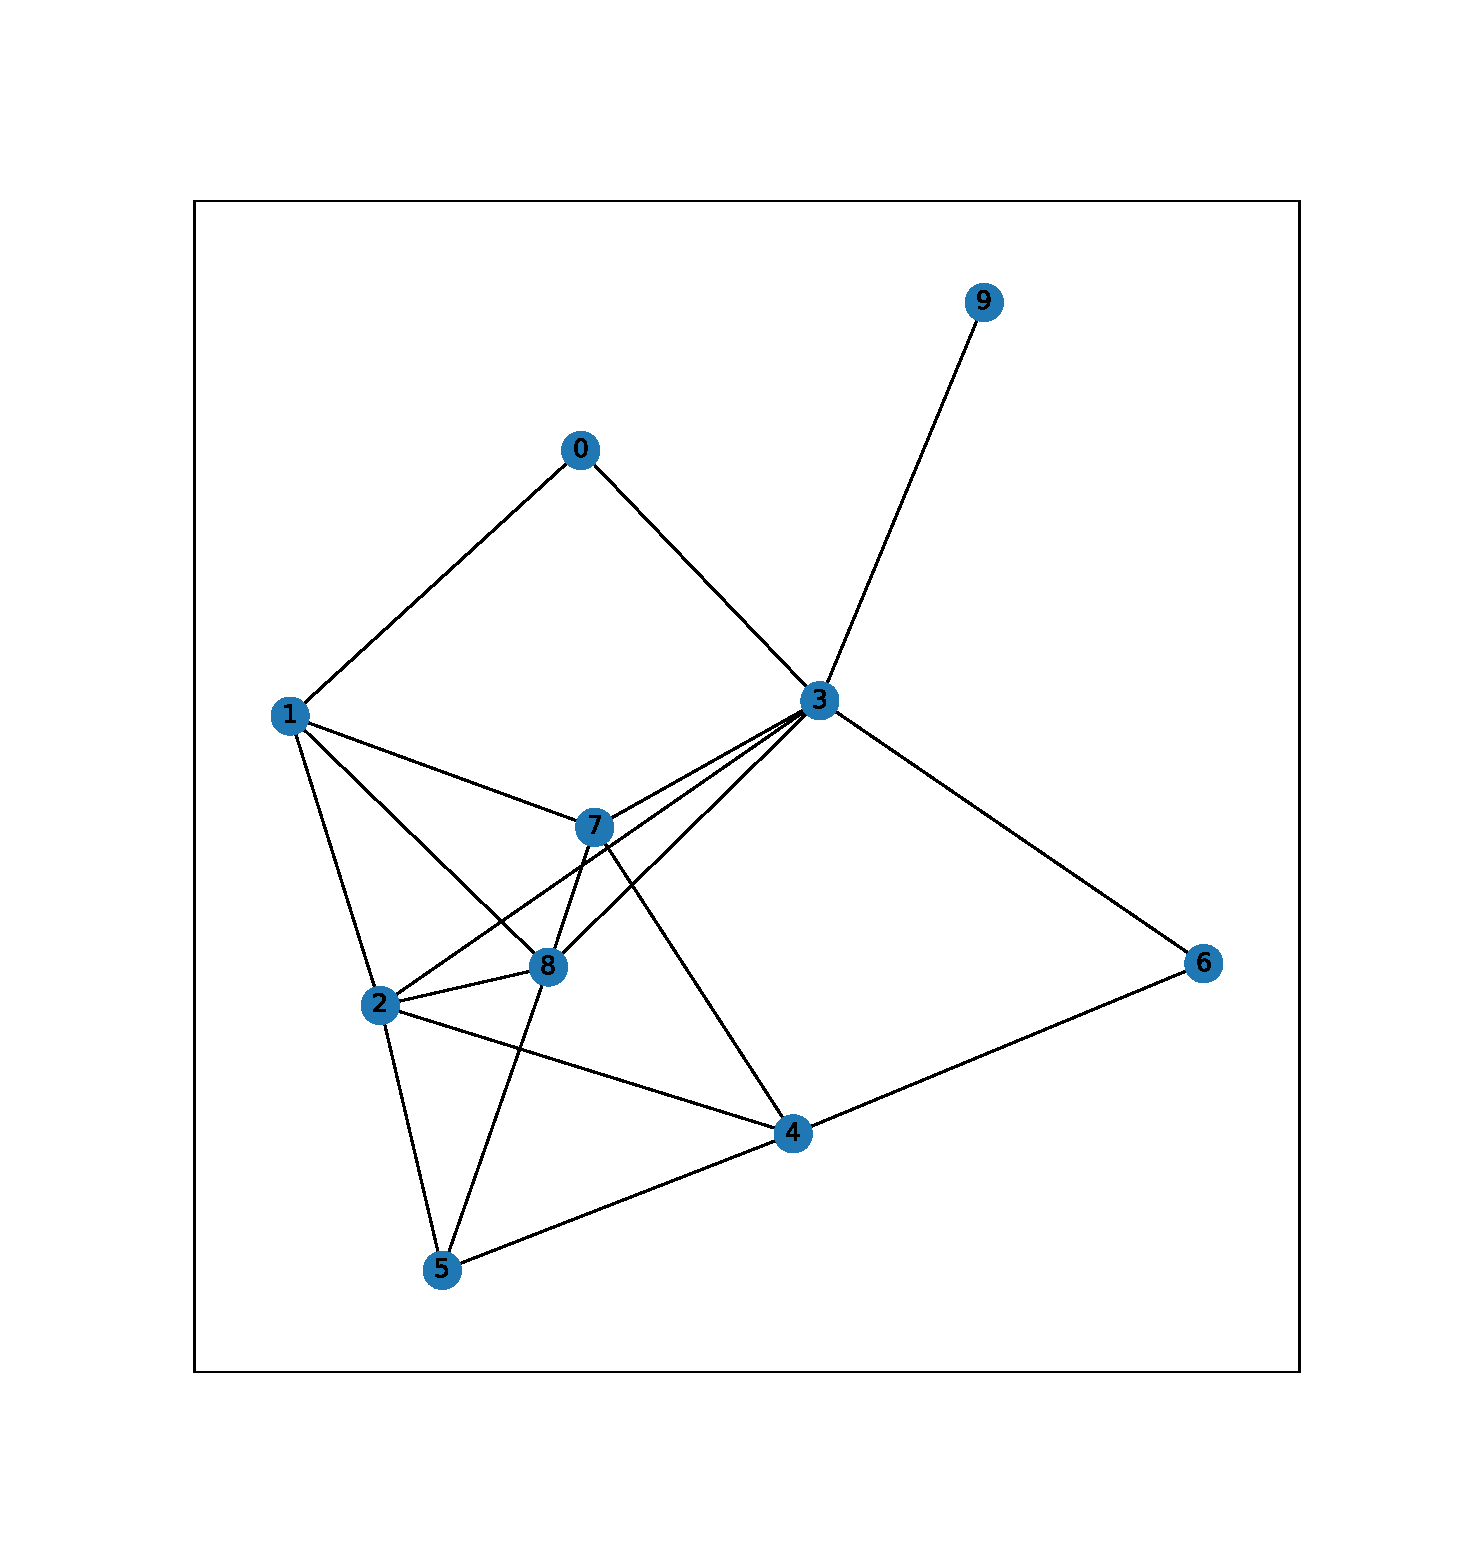
\includegraphics[height=0.7\textwidth,width=0.7\textwidth]{img/graph_2.eps}
\end{figure}

\begin{verbatim}
Duomenys:
n = 10 viršūnių, m = 18 briaunų
V = [0, 1, 2, 3, 4, 5, 6, 7, 8, 9]
E = [(0, 1), (0, 3), (1, 2), (1, 7), (1, 8), (2, 3), (2, 4), (2, 5), (2, 8),
(3, 6), (3, 7), (3, 8), (3, 9), (4, 5), (4, 6), (4, 7), (5, 8), (7, 8)]
Sugeneruotos maksimalios klikos:
[{0, 1}, {0, 3}, {8, 1, 2}, {8, 1, 7}, {8, 2, 3}, {8, 2, 5}, {2, 4, 5}, {4, 6},
{4, 7}, {3, 6}, {8, 3, 7}, {9, 3}]
\end{verbatim}

\subsection{Grafas 3}
\begin{figure}[H]
  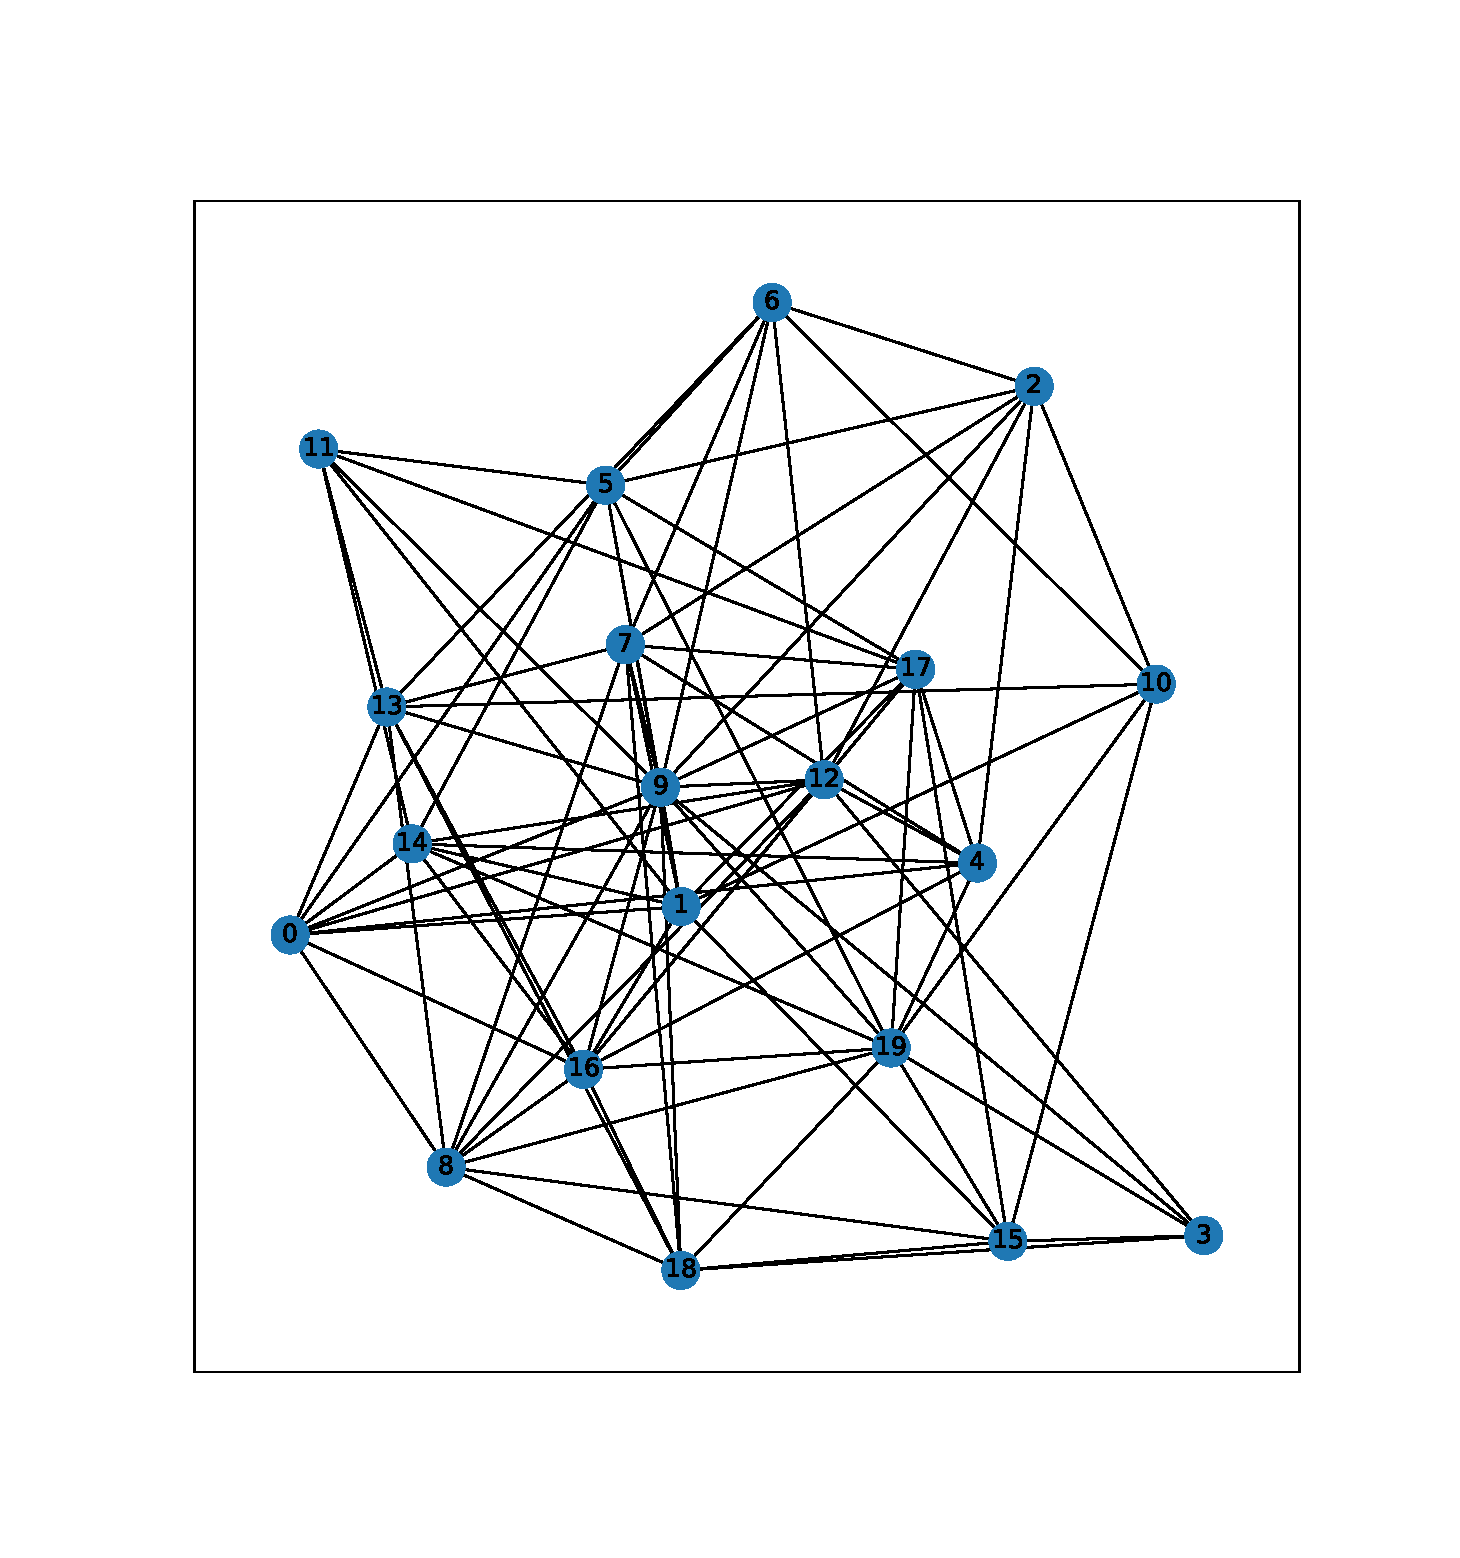
\includegraphics[height=0.7\textwidth,width=0.7\textwidth]{img/graph_3.eps}
\end{figure}

\begin{verbatim}
Duomenys:
n = 20 viršūnių, m = 89 briaunos
V =[0, 1, 2, 3, 4, 5, 6, 7, 8, 9, 10, 11, 12, 13, 14, 15, 16, 17, 18, 19]
E = [(0, 1), (0, 4), (0, 5), (0, 8), (0, 9), (0, 12), (0, 13), (0, 14),
(0, 16), (1, 5), (1, 7), (1, 9), (1, 10), (1, 11), (1, 14), (1, 15),
(1, 16), (1, 17), (2, 4), (2, 5), (2, 6), (2, 7), (2, 9), (2, 10), (2, 12),
(3, 9), (3, 12), (3, 15), (3, 18), (3, 19), (4, 7), (4, 12), (4, 14),
(4, 16), (4, 17), (4, 19), (5, 6), (5, 9), (5, 11), (5, 14), (5, 17),
(5, 19), (6, 7), (6, 9), (6, 10), (6, 12), (6, 13), (7, 8), (7, 9),
(7, 13), (7, 17), (7, 18), (8, 9), (8, 12), (8, 13), (8, 15), (8, 16),
(8, 18), (8, 19), (9, 11), (9, 12), (9, 13), (9, 16), (9, 17), (9, 18),
(9, 19), (10, 13), (10, 15), (10, 19), (11, 13), (11, 14), (11, 17),
(12, 14), (12, 16), (12, 17), (13, 16), (13, 18), (14, 16), (14, 19), 
(15, 17), (15, 18), (15, 19), (16, 17), (16, 18), (16, 19), (17, 19), (18, 19)]
Sugeneruotos maksimalios klikos:
[{0, 1, 9, 16}, {0, 1, 5, 9}, {0, 1, 14, 16}, {0, 1, 5, 14}, 
{1, 5, 9, 11, 17}, {1, 9, 17, 7}, {1, 17, 15}, {16, 1, 17, 9}, 
{1, 10, 15}, {1, 11, 5, 14}, {9, 2, 5, 6}, {9, 19, 5, 17}, 
{19, 5, 14}, {9, 2, 6, 7}, {2, 4, 7}, {17, 4, 7}, {9, 13, 6, 7}, 
{7, 8, 9, 13, 18}, {10, 2, 6}, {10, 19, 15}, {10, 13, 6}, {9, 11, 13}, 
{9, 3, 12}, {16, 17, 12, 4}, {2, 12, 4}, {0, 4, 12, 14, 16}, 
{9, 2, 12, 6}, {0, 8, 9, 12, 16}, {16, 9, 12, 17}, {0, 8, 9, 13, 16}, 
{8, 9, 13, 16, 18}, {8, 18, 19, 15}, {17, 19, 15}, {3, 18, 19, 15}, 
{8, 9, 16, 18, 19}, {19, 9, 18, 3}, {16, 17, 19, 9}, 
{16, 17, 19, 4}, {16, 19, 4, 14}]
\end{verbatim}

% Teoriškai išanalizuota ir praktiškai
\section{Sudėtingumo analizė}
\begin{centering}
\begin{tabular}{c c c c}
  \hline
  n & p & m & Vykd. laik. (s) \\
  \hline
  10  &  0.2   & 12 & 0.0009 \\
  30  &  0.5   & 210 & 0.0009 \\
  30  &  0.9   & 407 & 0.1619 \\
  50  &  0.2   & 240 & 0.0079 \\
  50  &  0.5   & 606 & 0.0797 \\
  50  &  0.9   & 1110 & 17.3075 \\
  100 &  0.2   & 949 & 0.0413 \\
  100 &  0.5   & 2441 & 1.4876 \\
  100 &  0.7   & 3480 & 61.9411 \\
  200 &  0.1   & 2023 & 0.0695 \\
  200 &  0.25  & 5084 & 0.7582 \\
  200 &  0.5  & 9903 & 51.0646 \\
  300 &  0.2   & 8750 & 1.0317 \\
  300 &  0.35   & 15757 & 18.9275 \\
  300 &  0.4   & 17950 & 51.146 \\
  500 &  0.1   & 12589 & 0.7203 \\
  500 &  0.2   & 25141 & 6.7183 \\
  500 &  0.3   & 37278 & 56.1880 \\
  \hline
\end{tabular}
\end{centering}

\begin{figure}[H]
\centering
\begin{tikzpicture}
\label{img:pvykd}
\begin{axis}[
    xmin = 100, xmax = 100000,
    xmode=log,
    ymode=log,
    ymin = 0, ymax = 100,
    nodes near coords,
    grid = both,
    minor tick num = 1,
    major grid style = {lightgray}, minor grid style = {lightgray!25},
    width = \textwidth, height = \textwidth,
    xlabel = {Briaunų Skaičius}, ylabel = {Vykdymo laikas (s)},
    legend cell align = {left}, legend pos = north west]
 
\addplot[smooth, thick, blue, mark=*] file[skip first] {data/vykd-50.dat};
\addplot[smooth, thick, red, mark=*] file[skip first] {data/vykd-100.dat};
\addplot[smooth, thick, pink, mark=*] file[skip first] {data/vykd-200.dat};
\addplot[smooth, thick, magenta, mark=*] file[skip first] {data/vykd-300.dat};
\addplot[smooth, thick, black, mark=*] file[skip first] {data/vykd-500.dat};

\legend{
  50 viršūnių,
  100 viršūnių,
  200 viršūnių,
  300 viršūnių,
  500 viršūnių
}
 
\end{axis}
\end{tikzpicture}
\end{figure}
Iš lentelės ir kreivių matome jog uždavinio sudėtingumas eksopentinis, kuo didesnis viršūnių kiekis - $n$, ir kuo arčiau briaunų kiekis $m$ yra arčiau grafo briaunų kiekio maksimumo $n * (n-1) / 2$, tuo šis algoritmas veikia lėčiau. Šis algoritmas kiekvieną kartą atradęs ne maksimalią kliką kviečia rekursyviai save dėl to paskaičiuoti sudėtingumą paeiliui - neįmanoma, žinome kad $3^{n/3}$ yra didžiausias maksimalių klikų kiekis bet kokiame $n$ viršūnių grafe. \cite{Moon1965OnCI}. Taip pat žinome, kad tai ir sutampa su šio algoritmo su atsparos tašku versija blogiausiu atvėju - $O(3^{n/3})$. \cite{Tomita2006TheWT}

\section{Išvados}
Taigi, pastebėjome kad algoritmo vykdymo laikas kinta tiek nuo viršūnių tiek nuo briaunų skaičiaus. Naivi šio algoritmo versija veiktu pakankamai lėčiau, taip pat šis algoritmas nepriklauso nuo rezultatų dydžio kaip kai kurie kiti algoritmai klikų problemai, jis taip pat nesuranda vienos maksimalios klikos per polinominį laiką, jis yra efektyviausias savo laiko kompleksiškumu blogiausiu atvėju ir praktikoje veikia greičiau negu kiti algoritmai.

\section{Programos naudojimo instrukcija}
\begin{verbatim}
Paleidžiame programa
$ python max_cliques.py
ir įvedame kintamuosius
Pvz: 
V = [1, 2, 3, 4, 5]
E = [(1, 2), (1, 3), (2, 3), (3, 4)]
\end{verbatim}

\printbibliography[heading=bibintoc] % Literatūros šaltiniai aprašomi

%\appendix  % Priedai

\end{document}
